\subsection{Superpixel flow}
\label{sec:suppix}

%\subsection{Problem definition}
%Superpixels and over segmentation techniques became a widely used pre-processing
 %stage for a large number of machine vision applications, after the
%original concept was introduced \cite{c1}. Superpixels are traditionally used as 
%performance booster for several other techniques. However, it is still mostly related to
%single frame processing \cite{c1}\cite{c10}\cite{c11}. In the search for
%consistency in superpixel labeling through video, some authors have proposed different 
%techniques, which go from simple extension to supervoxels\cite{c9}\cite{c11},
%to more complicated approaches \cite{c8}. These approaches, nonetheless, usually require a 
%global processing and knowledge of all (or several of) the video frames beforehand. 

As a preprocessing step in the object flow pipeline, we propose a superpixel matching technique which assumes a flowlike behavior in the image 
sequences (natural video), which can be used to track superpixels. 
%Some previous work have been done towards a
%superpixel based image comparison using the Earth Mover's Distance, by taking superpixels 
%as bins of a global histogram \cite{c2}. The label propagation or superpixel flow can be
%achieved with this technique as a byproduct, by selecting the superpixel in the second frame that 
%maximize the flow from each superpixel in the first frame.
%By taking into account superpixels computed separately in images, so the video process can be 
%performed with only two frames at a time, we move towards a more time efficient approach. 
This matching, however, has to comply with a set of constraints. 
Firstly, two correspondent superpixels should be similar in terms of some appearance
feature, which most likely depends on the way the superpixelization was performed (color, texture,
shape). Also, the superpixel flow  should maintain certain global regularity (at least for
superpixels that belong to the same object). %In this sense, it seems
%natural that the problem of superpixel flow could be solved with a discrete energy minimization
%procedure. 
If the size compactness of the superpixels is maintained,  it actually seems to 
share some of the properties of the optical flow problem, with the difference that the
smoothness is usually a very strong constraint for the last one. 
The strength of this smoothness prior relies not only in the nature of the problem, but also
because it gives better cues towards an easier-to-minimize global approach.

The objective of the superpixel flow is therefore to find the best labeling $l$ for every superpixel $p$
(with $l_p \in {0,1,...N-1}$) between a pair of frames ($I_{0}$,$I_{1}$), but holding a flow-like behaviour.

Thus, the superpixelization should maintain certain size homogeneity within a single frame. Some super
pixel techniques can cope with this requirement \cite{c9}\cite{c10}. For the experiments presented 
in this work, we prefer the SLIC method \cite{c9}, which usually gives
good results in terms of size homogeneity and compactness of the superpixelization. 
%The proposed steps to solve the propagation problem assume this requirement is hold. 
%For other kind of the techniques, other approaches should be followed.

%\addtolength{\textheight}{-3cm}   % This command serves to balance the column lengths
%%%%%%%%%%%%%%%%%%%%%%%%%%%%%%%%%%%%%%%%%%%%%%%%%%%%%%%%%%%%%%%%%%%%%%%%%%%%%%%%

%\subsection{Energy Formulation}

Inspired by a large number of optical flow and stereo techniques \cite{c7}\cite{c12}\cite{c13}, 
the superpixel flow can be modelled with pairwise Markov Random Fields. If
%the matching is performed with MAP inference, its posterior probability is: 
the matching is performed with MAP inference, its energy function extracted from the posterior probability is: 
%\begin{equation}
%P(l|I_0,I_1) = \displaystyle \prod_{p \in \Omega} \mathrm{e}^{-D_p(l_p;I_0,I_1)} 
%\prod_{p,q \in \mathcal{N}} \mathrm{e}^{-S_{p,q}(L_p;L_q)} 
%\label{eq_prob}
%\end{equation}

%With $l$ the set of labels of the super pixels in $I_0$,
%that match with those in $I_1$.
%$ \mathcal{N}_p $ is a neighborhood of the
%superpixel $p$, which defines its adjacency. Given this posterior probability,
%the equivalent energy function can be directly obtained
%by extracting the negative logarithm of the posterior,

\begin{equation}
E(l) = \displaystyle \sum_{p \in \Omega} D_p(L_p;I_0,I_1) +
\sum_{p,q \in \mathcal{N}} S_{p,q}(L_p,L_q)
\label{eq_energy}
\end{equation}

With $l$ the set of labels of the super pixels in $I_0$,
that match with those in $I_1$.
$ \mathcal{N} $ is a neighbourhood of the
superpixel $p$, which defines its adjacency. Given this posterior probability,
the equivalent energy function can be directly obtained
by extracting the negative logarithm of the posterior,

The terms $D$, and $S$ in (\ref{eq_energy}) stand for data term and spatial smoothness terms as they
are popularly known in the MRF literature. The first one determines how accurate is the labeling in terms
of consistency of the measured data (color, shape,etc.). In the classical optical flow formulation of this equation,
the data term corresponds to the pixel brightness conservation\cite{c7}\cite{c5}. However, as superpixels are a set
of similar (or somehow homogeneous) pixels, an adequate color based feature can be a low dimensional
color histogram. So $D$ can be written more precisely as the Hellinger distance between the histograms:

\begin{equation}
D_p(l_p;I_0,I_1) = \sqrt{ 1 - \frac{1}{\sqrt{\bar{h}(p)\bar{h}(p')N^2} } \sum_{i}\sqrt{h_{i}(p)h_{i}(p')} }
\label{eq_Dp}
\end{equation}

Where $h(p)$ and $h(p')$ are the histograms of the superpixel $p$ and its correspondent superpixel in the
second frame $I_1$. %The function $\rho$ is the Bhattacharyya distance. 
Note that the low dimensional histogram gives certain robustness against noise,
and slowly changing colors between frames. 

In the other hand, the spatial term is a penalty function for horizontal
and vertical changes of the vectors that have origin in the centroid of the superpixel of the first frame and
end in the centroid of the superpixel of the second frame.

\begin{equation}
S_{p,q}(l_p, l_q) = \lambda(p)
  \sqrt{\frac{|u_{p_c}-u_{q_c}|}{\|p_c-q_c\|}+ \frac{|v_{p_c}-v_{q_c}|}{\|p_c-q_c\|}}
\label{eq_Spq}
\end{equation}
\begin{center}
 where, $ \lambda(p) = (1 + \rho(h(p),h(q)))^2 $ \\
\end{center}

In (\ref{eq_Spq}) the operator $\rho$ is the Hellinger distance as used in the
data term (\ref{eq_Dp}). The histogram distance is nonetheless computed between superpixels $p$ and $q$, 
which belong to the same neighbourhood. The superpixels centroids are noted as $q_c$ and $p_c$, 
and $u$ and $v$ are the horizontal and vertical changes between centroids.
This term is usual in the MRF formulation and has a smoothing effect in superpixels that belong to the
same object. It has to be observed that when two close superpixels are different, thus, more probable to
belong to different objects within the image, the term $\lambda$ allows them to have
matches that do not hold the smoothness prior with the same strength. 
It has to be noted that the proposed energy function is highly non-convex.

%\subsection{Energy Minimization}

%A fair amount of work has been dedicated to discrete optimization techniques in computer vision,
%leading to well-defined and widely tested approaches to solve pairwise MRF\cite{c3}\cite{c4}.
%However, some of the approaches restrict the construction of the spatial term, and/or enforce
%limitations in the number of labels \cite{c3}.
%Because of the high amount of possible labels for  each superpixel in the proposed approach, the use of the
%Fusion Moves \cite{c7} technique seems to be well suited.
%This algorithm employs the Quadratic Pseudo-Boolean Optimization (QPBO), to combine
%incremental sets of proposal labelings, resulting in a semi-globally-optimal solution \cite{c4}.
%Thus, the minimization starts by proposing a set of possible solutions, and iteratively merges them with
%the QPBO technique. \\
%The candidate solutions depend on the problem to be solved. 
%For example, in stereo superpixel matching, some assumptions related to the cameras 
%layout can be made to generate solutions.
The Quadratic Pseudo-Boolean Optimization (QPBO) \cite{c3}\cite{c4} is used to minimize the proposed energy function, 
by merging a set of candidate matches for every superpixel in the first frame.
%In a more generic sense, other assumptions can be made towards candidate generation. 
For instance, for a given superpixel in the initial frame, the corresponding 
matching would be the most similar one in terms of color, shape, or the spatial distance. More candidate solutions can be added by defining a
neighbourhood in the second frame and select random pairs from every neighbourhood of every superpixel
in the first frame. %This is more suitable for problems where the images are extracted from the same video
%sequence. 
%To speed-up the minimization procedure, the QBPO properties can be exploted. For instance, the fusion of the
%proposed solutions is always guaranteed of lowest or equal energy than the two proposals. Thus, one could
%split the fusion procedure in several cores and build a hierarchichal chain as fusions of proposal are subsequently fused.

%   \begin{figure}[thpb]
%      \centering
%      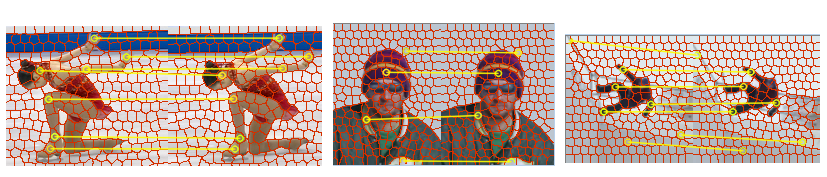
\includegraphics[width=1.00\textwidth]{images/matches.png}
%      \caption{The yellow lines show selected superpixel
%		matching between pairs of consecutive frames in a video
%		with the proposed method. The video frames go from right
%		to left.}
%      \label{figurelabel_matches}
%   \end{figure}

%\subsection{Matching results}
   \begin{figure}[thpb]
      \centering
      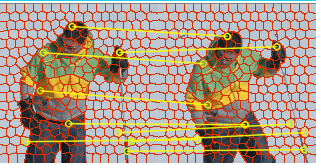
\includegraphics[width=0.70\textwidth]{../images/matches_snowshoes.png}
      \caption{The yellow lines show selected superpixel
		matching between a pair of distant frames in the Snow Shoes sequence.}
      \label{figurelabel_matchessnow}
   \end{figure}   
	\setlength{\belowcaptionskip}{-10pt}
%The Fig. \ref{figurelabel_matches} shows some examples of superpixel matching with the presented method. 
%It can be seen that the matching performs well even in difficult cases, like the hands in the top row. It has to be noted
%as well that even in superpixels where there is a lack of texture, there is correct matching. This seems to be
%the effect of enforcing the regularization between superpixels that are close, but are also similar to
%each other.
 
% Moreover, unlike most of the optical flow methods, superpixel flow extends 
 %naturally for more distant frames. 
The Fig. \ref{figurelabel_matchessnow} shows
 results for large separations between frames. % without tweaking or adjusting any parameters. 
For this case, however, the matches in the textureless part of the scene
 are mostly invalids. Though this is expected because of the aperture problem and
 heavy occlusions.
